
% Default to the notebook output style

    


% Inherit from the specified cell style.




    
\documentclass[11pt]{article}

    
    \author{Daniel Fraser, Peter Laskai}
    \usepackage[T1]{fontenc}
    % Nicer default font (+ math font) than Computer Modern for most use cases
    \usepackage{mathpazo}

    % Basic figure setup, for now with no caption control since it's done
    % automatically by Pandoc (which extracts ![](path) syntax from Markdown).
    \usepackage{graphicx}
    % We will generate all images so they have a width \maxwidth. This means
    % that they will get their normal width if they fit onto the page, but
    % are scaled down if they would overflow the margins.
    \makeatletter
    \def\maxwidth{\ifdim\Gin@nat@width>\linewidth\linewidth
    \else\Gin@nat@width\fi}
    \makeatother
    \let\Oldincludegraphics\includegraphics
    % Set max figure width to be 80% of text width, for now hardcoded.
    \renewcommand{\includegraphics}[1]{\Oldincludegraphics[width=.8\maxwidth]{#1}}
    % Ensure that by default, figures have no caption (until we provide a
    % proper Figure object with a Caption API and a way to capture that
    % in the conversion process - todo).
    \usepackage{caption}
    \DeclareCaptionLabelFormat{nolabel}{}
    \captionsetup{labelformat=nolabel}

    \usepackage{adjustbox} % Used to constrain images to a maximum size 
    \usepackage{xcolor} % Allow colors to be defined
    \usepackage{enumerate} % Needed for markdown enumerations to work
    \usepackage{geometry} % Used to adjust the document margins
    \usepackage{amsmath} % Equations
    \usepackage{amssymb} % Equations
    \usepackage{textcomp} % defines textquotesingle
    % Hack from http://tex.stackexchange.com/a/47451/13684:
    \AtBeginDocument{%
        \def\PYZsq{\textquotesingle}% Upright quotes in Pygmentized code
    }
    \usepackage{upquote} % Upright quotes for verbatim code
    \usepackage{eurosym} % defines \euro
    \usepackage[mathletters]{ucs} % Extended unicode (utf-8) support
    \usepackage[utf8x]{inputenc} % Allow utf-8 characters in the tex document
    \usepackage{fancyvrb} % verbatim replacement that allows latex
    \usepackage{grffile} % extends the file name processing of package graphics 
                         % to support a larger range 
    % The hyperref package gives us a pdf with properly built
    % internal navigation ('pdf bookmarks' for the table of contents,
    % internal cross-reference links, web links for URLs, etc.)
    \usepackage{hyperref}
    \usepackage{longtable} % longtable support required by pandoc >1.10
    \usepackage{booktabs}  % table support for pandoc > 1.12.2
    \usepackage[inline]{enumitem} % IRkernel/repr support (it uses the enumerate* environment)
    \usepackage[normalem]{ulem} % ulem is needed to support strikethroughs (\sout)
                                % normalem makes italics be italics, not underlines
    \usepackage{float}

    
    
    % Colors for the hyperref package
    \definecolor{urlcolor}{rgb}{0,.145,.698}
    \definecolor{linkcolor}{rgb}{.71,0.21,0.01}
    \definecolor{citecolor}{rgb}{.12,.54,.11}

    % ANSI colors
    \definecolor{ansi-black}{HTML}{3E424D}
    \definecolor{ansi-black-intense}{HTML}{282C36}
    \definecolor{ansi-red}{HTML}{E75C58}
    \definecolor{ansi-red-intense}{HTML}{B22B31}
    \definecolor{ansi-green}{HTML}{00A250}
    \definecolor{ansi-green-intense}{HTML}{007427}
    \definecolor{ansi-yellow}{HTML}{DDB62B}
    \definecolor{ansi-yellow-intense}{HTML}{B27D12}
    \definecolor{ansi-blue}{HTML}{208FFB}
    \definecolor{ansi-blue-intense}{HTML}{0065CA}
    \definecolor{ansi-magenta}{HTML}{D160C4}
    \definecolor{ansi-magenta-intense}{HTML}{A03196}
    \definecolor{ansi-cyan}{HTML}{60C6C8}
    \definecolor{ansi-cyan-intense}{HTML}{258F8F}
    \definecolor{ansi-white}{HTML}{C5C1B4}
    \definecolor{ansi-white-intense}{HTML}{A1A6B2}

    % commands and environments needed by pandoc snippets
    % extracted from the output of `pandoc -s`
    \providecommand{\tightlist}{%
      \setlength{\itemsep}{0pt}\setlength{\parskip}{0pt}}
    \DefineVerbatimEnvironment{Highlighting}{Verbatim}{commandchars=\\\{\}}
    % Add ',fontsize=\small' for more characters per line
    \newenvironment{Shaded}{}{}
    \newcommand{\KeywordTok}[1]{\textcolor[rgb]{0.00,0.44,0.13}{\textbf{{#1}}}}
    \newcommand{\DataTypeTok}[1]{\textcolor[rgb]{0.56,0.13,0.00}{{#1}}}
    \newcommand{\DecValTok}[1]{\textcolor[rgb]{0.25,0.63,0.44}{{#1}}}
    \newcommand{\BaseNTok}[1]{\textcolor[rgb]{0.25,0.63,0.44}{{#1}}}
    \newcommand{\FloatTok}[1]{\textcolor[rgb]{0.25,0.63,0.44}{{#1}}}
    \newcommand{\CharTok}[1]{\textcolor[rgb]{0.25,0.44,0.63}{{#1}}}
    \newcommand{\StringTok}[1]{\textcolor[rgb]{0.25,0.44,0.63}{{#1}}}
    \newcommand{\CommentTok}[1]{\textcolor[rgb]{0.38,0.63,0.69}{\textit{{#1}}}}
    \newcommand{\OtherTok}[1]{\textcolor[rgb]{0.00,0.44,0.13}{{#1}}}
    \newcommand{\AlertTok}[1]{\textcolor[rgb]{1.00,0.00,0.00}{\textbf{{#1}}}}
    \newcommand{\FunctionTok}[1]{\textcolor[rgb]{0.02,0.16,0.49}{{#1}}}
    \newcommand{\RegionMarkerTok}[1]{{#1}}
    \newcommand{\ErrorTok}[1]{\textcolor[rgb]{1.00,0.00,0.00}{\textbf{{#1}}}}
    \newcommand{\NormalTok}[1]{{#1}}
    
    % Additional commands for more recent versions of Pandoc
    \newcommand{\ConstantTok}[1]{\textcolor[rgb]{0.53,0.00,0.00}{{#1}}}
    \newcommand{\SpecialCharTok}[1]{\textcolor[rgb]{0.25,0.44,0.63}{{#1}}}
    \newcommand{\VerbatimStringTok}[1]{\textcolor[rgb]{0.25,0.44,0.63}{{#1}}}
    \newcommand{\SpecialStringTok}[1]{\textcolor[rgb]{0.73,0.40,0.53}{{#1}}}
    \newcommand{\ImportTok}[1]{{#1}}
    \newcommand{\DocumentationTok}[1]{\textcolor[rgb]{0.73,0.13,0.13}{\textit{{#1}}}}
    \newcommand{\AnnotationTok}[1]{\textcolor[rgb]{0.38,0.63,0.69}{\textbf{\textit{{#1}}}}}
    \newcommand{\CommentVarTok}[1]{\textcolor[rgb]{0.38,0.63,0.69}{\textbf{\textit{{#1}}}}}
    \newcommand{\VariableTok}[1]{\textcolor[rgb]{0.10,0.09,0.49}{{#1}}}
    \newcommand{\ControlFlowTok}[1]{\textcolor[rgb]{0.00,0.44,0.13}{\textbf{{#1}}}}
    \newcommand{\OperatorTok}[1]{\textcolor[rgb]{0.40,0.40,0.40}{{#1}}}
    \newcommand{\BuiltInTok}[1]{{#1}}
    \newcommand{\ExtensionTok}[1]{{#1}}
    \newcommand{\PreprocessorTok}[1]{\textcolor[rgb]{0.74,0.48,0.00}{{#1}}}
    \newcommand{\AttributeTok}[1]{\textcolor[rgb]{0.49,0.56,0.16}{{#1}}}
    \newcommand{\InformationTok}[1]{\textcolor[rgb]{0.38,0.63,0.69}{\textbf{\textit{{#1}}}}}
    \newcommand{\WarningTok}[1]{\textcolor[rgb]{0.38,0.63,0.69}{\textbf{\textit{{#1}}}}}
    
    
    % Define a nice break command that doesn't care if a line doesn't already
    % exist.
    \def\br{\hspace*{\fill} \\* }
    % Math Jax compatability definitions
    \def\gt{>}
    \def\lt{<}
    % Document parameters
    \title{Final Report: Programming Languages and
    	GitHub}
    
    
    

    % Pygments definitions
    
\makeatletter
\def\PY@reset{\let\PY@it=\relax \let\PY@bf=\relax%
    \let\PY@ul=\relax \let\PY@tc=\relax%
    \let\PY@bc=\relax \let\PY@ff=\relax}
\def\PY@tok#1{\csname PY@tok@#1\endcsname}
\def\PY@toks#1+{\ifx\relax#1\empty\else%
    \PY@tok{#1}\expandafter\PY@toks\fi}
\def\PY@do#1{\PY@bc{\PY@tc{\PY@ul{%
    \PY@it{\PY@bf{\PY@ff{#1}}}}}}}
\def\PY#1#2{\PY@reset\PY@toks#1+\relax+\PY@do{#2}}

\expandafter\def\csname PY@tok@w\endcsname{\def\PY@tc##1{\textcolor[rgb]{0.73,0.73,0.73}{##1}}}
\expandafter\def\csname PY@tok@c\endcsname{\let\PY@it=\textit\def\PY@tc##1{\textcolor[rgb]{0.25,0.50,0.50}{##1}}}
\expandafter\def\csname PY@tok@cp\endcsname{\def\PY@tc##1{\textcolor[rgb]{0.74,0.48,0.00}{##1}}}
\expandafter\def\csname PY@tok@k\endcsname{\let\PY@bf=\textbf\def\PY@tc##1{\textcolor[rgb]{0.00,0.50,0.00}{##1}}}
\expandafter\def\csname PY@tok@kp\endcsname{\def\PY@tc##1{\textcolor[rgb]{0.00,0.50,0.00}{##1}}}
\expandafter\def\csname PY@tok@kt\endcsname{\def\PY@tc##1{\textcolor[rgb]{0.69,0.00,0.25}{##1}}}
\expandafter\def\csname PY@tok@o\endcsname{\def\PY@tc##1{\textcolor[rgb]{0.40,0.40,0.40}{##1}}}
\expandafter\def\csname PY@tok@ow\endcsname{\let\PY@bf=\textbf\def\PY@tc##1{\textcolor[rgb]{0.67,0.13,1.00}{##1}}}
\expandafter\def\csname PY@tok@nb\endcsname{\def\PY@tc##1{\textcolor[rgb]{0.00,0.50,0.00}{##1}}}
\expandafter\def\csname PY@tok@nf\endcsname{\def\PY@tc##1{\textcolor[rgb]{0.00,0.00,1.00}{##1}}}
\expandafter\def\csname PY@tok@nc\endcsname{\let\PY@bf=\textbf\def\PY@tc##1{\textcolor[rgb]{0.00,0.00,1.00}{##1}}}
\expandafter\def\csname PY@tok@nn\endcsname{\let\PY@bf=\textbf\def\PY@tc##1{\textcolor[rgb]{0.00,0.00,1.00}{##1}}}
\expandafter\def\csname PY@tok@ne\endcsname{\let\PY@bf=\textbf\def\PY@tc##1{\textcolor[rgb]{0.82,0.25,0.23}{##1}}}
\expandafter\def\csname PY@tok@nv\endcsname{\def\PY@tc##1{\textcolor[rgb]{0.10,0.09,0.49}{##1}}}
\expandafter\def\csname PY@tok@no\endcsname{\def\PY@tc##1{\textcolor[rgb]{0.53,0.00,0.00}{##1}}}
\expandafter\def\csname PY@tok@nl\endcsname{\def\PY@tc##1{\textcolor[rgb]{0.63,0.63,0.00}{##1}}}
\expandafter\def\csname PY@tok@ni\endcsname{\let\PY@bf=\textbf\def\PY@tc##1{\textcolor[rgb]{0.60,0.60,0.60}{##1}}}
\expandafter\def\csname PY@tok@na\endcsname{\def\PY@tc##1{\textcolor[rgb]{0.49,0.56,0.16}{##1}}}
\expandafter\def\csname PY@tok@nt\endcsname{\let\PY@bf=\textbf\def\PY@tc##1{\textcolor[rgb]{0.00,0.50,0.00}{##1}}}
\expandafter\def\csname PY@tok@nd\endcsname{\def\PY@tc##1{\textcolor[rgb]{0.67,0.13,1.00}{##1}}}
\expandafter\def\csname PY@tok@s\endcsname{\def\PY@tc##1{\textcolor[rgb]{0.73,0.13,0.13}{##1}}}
\expandafter\def\csname PY@tok@sd\endcsname{\let\PY@it=\textit\def\PY@tc##1{\textcolor[rgb]{0.73,0.13,0.13}{##1}}}
\expandafter\def\csname PY@tok@si\endcsname{\let\PY@bf=\textbf\def\PY@tc##1{\textcolor[rgb]{0.73,0.40,0.53}{##1}}}
\expandafter\def\csname PY@tok@se\endcsname{\let\PY@bf=\textbf\def\PY@tc##1{\textcolor[rgb]{0.73,0.40,0.13}{##1}}}
\expandafter\def\csname PY@tok@sr\endcsname{\def\PY@tc##1{\textcolor[rgb]{0.73,0.40,0.53}{##1}}}
\expandafter\def\csname PY@tok@ss\endcsname{\def\PY@tc##1{\textcolor[rgb]{0.10,0.09,0.49}{##1}}}
\expandafter\def\csname PY@tok@sx\endcsname{\def\PY@tc##1{\textcolor[rgb]{0.00,0.50,0.00}{##1}}}
\expandafter\def\csname PY@tok@m\endcsname{\def\PY@tc##1{\textcolor[rgb]{0.40,0.40,0.40}{##1}}}
\expandafter\def\csname PY@tok@gh\endcsname{\let\PY@bf=\textbf\def\PY@tc##1{\textcolor[rgb]{0.00,0.00,0.50}{##1}}}
\expandafter\def\csname PY@tok@gu\endcsname{\let\PY@bf=\textbf\def\PY@tc##1{\textcolor[rgb]{0.50,0.00,0.50}{##1}}}
\expandafter\def\csname PY@tok@gd\endcsname{\def\PY@tc##1{\textcolor[rgb]{0.63,0.00,0.00}{##1}}}
\expandafter\def\csname PY@tok@gi\endcsname{\def\PY@tc##1{\textcolor[rgb]{0.00,0.63,0.00}{##1}}}
\expandafter\def\csname PY@tok@gr\endcsname{\def\PY@tc##1{\textcolor[rgb]{1.00,0.00,0.00}{##1}}}
\expandafter\def\csname PY@tok@ge\endcsname{\let\PY@it=\textit}
\expandafter\def\csname PY@tok@gs\endcsname{\let\PY@bf=\textbf}
\expandafter\def\csname PY@tok@gp\endcsname{\let\PY@bf=\textbf\def\PY@tc##1{\textcolor[rgb]{0.00,0.00,0.50}{##1}}}
\expandafter\def\csname PY@tok@go\endcsname{\def\PY@tc##1{\textcolor[rgb]{0.53,0.53,0.53}{##1}}}
\expandafter\def\csname PY@tok@gt\endcsname{\def\PY@tc##1{\textcolor[rgb]{0.00,0.27,0.87}{##1}}}
\expandafter\def\csname PY@tok@err\endcsname{\def\PY@bc##1{\setlength{\fboxsep}{0pt}\fcolorbox[rgb]{1.00,0.00,0.00}{1,1,1}{\strut ##1}}}
\expandafter\def\csname PY@tok@kc\endcsname{\let\PY@bf=\textbf\def\PY@tc##1{\textcolor[rgb]{0.00,0.50,0.00}{##1}}}
\expandafter\def\csname PY@tok@kd\endcsname{\let\PY@bf=\textbf\def\PY@tc##1{\textcolor[rgb]{0.00,0.50,0.00}{##1}}}
\expandafter\def\csname PY@tok@kn\endcsname{\let\PY@bf=\textbf\def\PY@tc##1{\textcolor[rgb]{0.00,0.50,0.00}{##1}}}
\expandafter\def\csname PY@tok@kr\endcsname{\let\PY@bf=\textbf\def\PY@tc##1{\textcolor[rgb]{0.00,0.50,0.00}{##1}}}
\expandafter\def\csname PY@tok@bp\endcsname{\def\PY@tc##1{\textcolor[rgb]{0.00,0.50,0.00}{##1}}}
\expandafter\def\csname PY@tok@fm\endcsname{\def\PY@tc##1{\textcolor[rgb]{0.00,0.00,1.00}{##1}}}
\expandafter\def\csname PY@tok@vc\endcsname{\def\PY@tc##1{\textcolor[rgb]{0.10,0.09,0.49}{##1}}}
\expandafter\def\csname PY@tok@vg\endcsname{\def\PY@tc##1{\textcolor[rgb]{0.10,0.09,0.49}{##1}}}
\expandafter\def\csname PY@tok@vi\endcsname{\def\PY@tc##1{\textcolor[rgb]{0.10,0.09,0.49}{##1}}}
\expandafter\def\csname PY@tok@vm\endcsname{\def\PY@tc##1{\textcolor[rgb]{0.10,0.09,0.49}{##1}}}
\expandafter\def\csname PY@tok@sa\endcsname{\def\PY@tc##1{\textcolor[rgb]{0.73,0.13,0.13}{##1}}}
\expandafter\def\csname PY@tok@sb\endcsname{\def\PY@tc##1{\textcolor[rgb]{0.73,0.13,0.13}{##1}}}
\expandafter\def\csname PY@tok@sc\endcsname{\def\PY@tc##1{\textcolor[rgb]{0.73,0.13,0.13}{##1}}}
\expandafter\def\csname PY@tok@dl\endcsname{\def\PY@tc##1{\textcolor[rgb]{0.73,0.13,0.13}{##1}}}
\expandafter\def\csname PY@tok@s2\endcsname{\def\PY@tc##1{\textcolor[rgb]{0.73,0.13,0.13}{##1}}}
\expandafter\def\csname PY@tok@sh\endcsname{\def\PY@tc##1{\textcolor[rgb]{0.73,0.13,0.13}{##1}}}
\expandafter\def\csname PY@tok@s1\endcsname{\def\PY@tc##1{\textcolor[rgb]{0.73,0.13,0.13}{##1}}}
\expandafter\def\csname PY@tok@mb\endcsname{\def\PY@tc##1{\textcolor[rgb]{0.40,0.40,0.40}{##1}}}
\expandafter\def\csname PY@tok@mf\endcsname{\def\PY@tc##1{\textcolor[rgb]{0.40,0.40,0.40}{##1}}}
\expandafter\def\csname PY@tok@mh\endcsname{\def\PY@tc##1{\textcolor[rgb]{0.40,0.40,0.40}{##1}}}
\expandafter\def\csname PY@tok@mi\endcsname{\def\PY@tc##1{\textcolor[rgb]{0.40,0.40,0.40}{##1}}}
\expandafter\def\csname PY@tok@il\endcsname{\def\PY@tc##1{\textcolor[rgb]{0.40,0.40,0.40}{##1}}}
\expandafter\def\csname PY@tok@mo\endcsname{\def\PY@tc##1{\textcolor[rgb]{0.40,0.40,0.40}{##1}}}
\expandafter\def\csname PY@tok@ch\endcsname{\let\PY@it=\textit\def\PY@tc##1{\textcolor[rgb]{0.25,0.50,0.50}{##1}}}
\expandafter\def\csname PY@tok@cm\endcsname{\let\PY@it=\textit\def\PY@tc##1{\textcolor[rgb]{0.25,0.50,0.50}{##1}}}
\expandafter\def\csname PY@tok@cpf\endcsname{\let\PY@it=\textit\def\PY@tc##1{\textcolor[rgb]{0.25,0.50,0.50}{##1}}}
\expandafter\def\csname PY@tok@c1\endcsname{\let\PY@it=\textit\def\PY@tc##1{\textcolor[rgb]{0.25,0.50,0.50}{##1}}}
\expandafter\def\csname PY@tok@cs\endcsname{\let\PY@it=\textit\def\PY@tc##1{\textcolor[rgb]{0.25,0.50,0.50}{##1}}}

\def\PYZbs{\char`\\}
\def\PYZus{\char`\_}
\def\PYZob{\char`\{}
\def\PYZcb{\char`\}}
\def\PYZca{\char`\^}
\def\PYZam{\char`\&}
\def\PYZlt{\char`\<}
\def\PYZgt{\char`\>}
\def\PYZsh{\char`\#}
\def\PYZpc{\char`\%}
\def\PYZdl{\char`\$}
\def\PYZhy{\char`\-}
\def\PYZsq{\char`\'}
\def\PYZdq{\char`\"}
\def\PYZti{\char`\~}
% for compatibility with earlier versions
\def\PYZat{@}
\def\PYZlb{[}
\def\PYZrb{]}
\makeatother


    % Exact colors from NB
    \definecolor{incolor}{rgb}{0.0, 0.0, 0.5}
    \definecolor{outcolor}{rgb}{0.545, 0.0, 0.0}



    
    % Prevent overflowing lines due to hard-to-break entities
    \sloppy 
    % Setup hyperref package
    \hypersetup{
      breaklinks=true,  % so long urls are correctly broken across lines
      colorlinks=true,
      urlcolor=urlcolor,
      linkcolor=linkcolor,
      citecolor=citecolor,
      }
    % Slightly bigger margins than the latex defaults
    
    \geometry{verbose,tmargin=1in,bmargin=1in,lmargin=1in,rmargin=1in}
    
    

    \begin{document}
    
    
    \maketitle
    


    \section{Describe project goals and why it is
interesting}\label{describe-project-goals-and-why-it-is-interesting}

We plan to use this data to predict which languages are being used, what
they're being used for (commercial, fun, etc). The data behind Github is
fascinating because it is one the most used version control software out
there and allows the public to see the trend of languages throughout the
years and see what type of projects people create, and how they
collaborate with one another.

    \section{Describe data collection/source of data, data format, data
preprocessing}\label{describe-data-collectionsource-of-data-data-format-data-preprocessing}

This dataset gives us info on what languages are used, its files
(including their contents) and their size along with info on commits. We
will use a combination of the data from bigquery along with using
Github's official api using javascript. Bigquery's data is listed as
tables, while the api will give us info in the form of an API response
as json file. With bigquery, we have to eliminate rows that have a date
before the creation of github (which is about 0.04\% (10 million) which
is most likely an error from importing data to bigQuery) of the total
rows. With the api, we eliminate some of the redundant information such
as owner of repo (since unless you're searching, you get the repo based
off the username).

One of our data collection source was Octokit's
\href{https://github.com/octokit/rest.js}{rest.js}, a JavaScript based
API scraper tool adopted by the GitHub team. From there we could access
a large amount github data arranging from, user info, repository
details, gists, issues, and pull requests from 24 million users.This is
an example of a ``query'' using rest.js:

\begin{verbatim}
//This specific function gets all the info of JavaFXMusicLibrary repository from user PrL327
octokit.repos.get({
  owner: 'prl327',
  repo: 'JavaFXMusicLibrary'
}).then(({data}) => {
  console.log(data);
}); 
\end{verbatim}

Right now since we can only evaluate data that is public like public
organizations and public repos, we had to put a safeguard in which we
return 0, which in the end we filter out. We also have to worry about
hitting the query limit for the api which is 1000 queries a hour. We
actually combined the use of BigQuery and Rest.js in one example. We had
a csv file which contained two columns for username and repository, with
about 10,000 rows. to easily process that csv file through our query we
needed to convert it to a JSON for easy parsing. For this we used csv a
node library and it's resepective functions to do the conversion, it
produce an object like such:
\texttt{\{\ \ \ \ \ \ "User":\ "prl327",\ \ \ \ \ \ "Repository":\ "JavaFXMusicLibrary"\ \ \}}
And so on for 10,000 more user/repo combinations.

    \section{Describe contents of data in detail (write code to analyse and
visualize
it)}\label{describe-contents-of-data-in-detail-write-code-to-analyse-and-visualize-it}

    \subsubsection{Why Github?}\label{why-github}

Githhub is a very active community with millions of user constantly
collaborating and contributing to projects. We gathered contributer data
using the github api since bigquery doesn't have any tables with
information on contributors. We were surpised to find that most of the
projects hosted there on github are only worked by only one person.

    \begin{Verbatim}[commandchars=\\\{\}]
{\color{incolor}In [{\color{incolor}1}]:} repos \PY{o}{\PYZlt{}\PYZhy{}} read.csv\PY{p}{(}\PY{l+s}{\PYZdq{}}\PY{l+s}{repos.csv\PYZdq{}}\PY{p}{,} header \PY{o}{=} \PY{k+kc}{TRUE}\PY{p}{)}
        hist\PY{p}{(}repos\PY{o}{\PYZdl{}}\PY{k+kp}{contributors}\PY{p}{[}repos\PY{o}{\PYZdl{}}contributors \PY{o}{\PYZgt{}} \PY{l+m}{0} \PY{o}{\PYZam{}} repos\PY{o}{\PYZdl{}}contributors \PY{o}{\PYZlt{}} \PY{l+m}{30}\PY{p}{]}\PY{p}{,} \PY{l+m}{10}\PY{p}{,}
             col \PY{o}{=} rainbow\PY{p}{(}\PY{l+m}{20}\PY{p}{)}\PY{p}{,} xlab \PY{o}{=} \PY{l+s}{\PYZdq{}}\PY{l+s}{Number of contributors\PYZdq{}}\PY{p}{,} main \PY{o}{=} \PY{l+s}{\PYZdq{}}\PY{l+s}{Frequency of number of contributors\PYZbs{}n(for repositories with less than 30 contributors)\PYZdq{}}\PY{p}{)}
\end{Verbatim}


    \begin{center}
    \adjustimage{max size={0.9\linewidth}{0.9\paperheight}}{output_5_0.png}
    \end{center}
    { \hspace*{\fill} \\}
    
    \subsection{Languages Used the most}\label{languages-used-the-most}

    We filtered out the \texttt{languages} table from bigquery's dataset to
only show the top 15 languages by occurrences:

\begin{Shaded}
\begin{Highlighting}[]
\KeywordTok{SELECT}
\NormalTok{  name,}
  \FunctionTok{COUNT}\NormalTok{(*) }\KeywordTok{AS}\NormalTok{ occurences}
\KeywordTok{FROM}
\NormalTok{  `bigquery-public-data.github_repos.languages` }\KeywordTok{AS}\NormalTok{ l,}
\NormalTok{  UNNEST(l.LANGUAGE)}
\KeywordTok{GROUP} \KeywordTok{BY}
\NormalTok{  name}
\KeywordTok{ORDER} \KeywordTok{BY}
\NormalTok{  occurences }\KeywordTok{DESC}
  \KeywordTok{limit} \DecValTok{15}
\end{Highlighting}
\end{Shaded}

\begin{figure}[H]
\centering
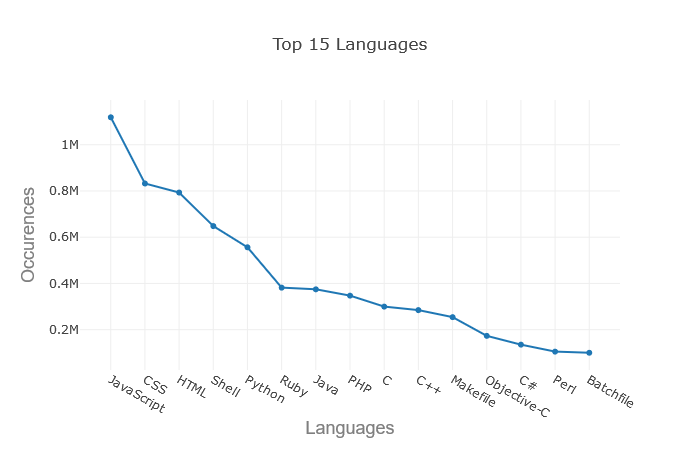
\includegraphics{newplot3.png}
\caption{}
\end{figure}

    Unsuprisingly the biggest languages used in the world round up the top
15 used languages in Github. JavaScript takes the top with 1.2 Million
Occurrences in our dataset. Javascript is also a heavily modified
langauage with sub languages like JQuery, NodeJS, ReactJS, and
AngularJS.

    \subsection{Languages Used the Least}\label{languages-used-the-least}

    We filtered out the \texttt{languages} table from bigquery's dataset to
only show the 15 languages with the lowest occurrences:

\begin{Shaded}
\begin{Highlighting}[]
	\KeywordTok{SELECT}
	\NormalTok{  name,}
	\FunctionTok{COUNT}\NormalTok{(*) }\KeywordTok{AS}\NormalTok{ occurences}
	\KeywordTok{FROM}
	\NormalTok{  `bigquery-public-data.github_repos.languages` }\KeywordTok{AS}\NormalTok{ l,}
	\NormalTok{  UNNEST(l.LANGUAGE)}
	\KeywordTok{GROUP} \KeywordTok{BY}
	\NormalTok{  name}
	\KeywordTok{ORDER} \KeywordTok{BY}
	\NormalTok{  occurences }
	\KeywordTok{limit} \DecValTok{15}
\end{Highlighting}
\end{Shaded}


\begin{figure}[H]
\centering
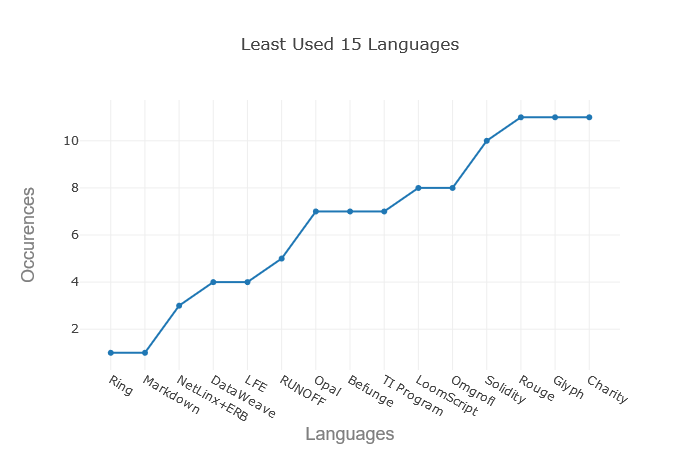
\includegraphics{newplot2.png}
\caption{}
\end{figure}

    Processing through the data produced some interesting results. First to
note Markdown is noted as one of the lead used but when visiting GitHub
you see README.md in almost every repo. In this case the Dataset from
GoogleBigquery does not count README files when referencing language
data. Ring is a language we have actually never heard before. If you
search GitHub you'll find only 18 repositories that use Ring. The
lanuage is a mult-paradigmn language that can be used for apps on
multiple OSes and with a GCC compiler.

    \subsection{15 Languages using the most
bytes}\label{languages-using-the-most-bytes}

    For bytes we continued analyzed the dataset's \texttt{langauges} table
this time getting the sum of bytes:

\begin{Shaded}
\begin{Highlighting}[]
\KeywordTok{SELECT}
\NormalTok{  name,}
  \FunctionTok{SUM}\NormalTok{(bytes) }\KeywordTok{AS}\NormalTok{ totalBytes}
\KeywordTok{FROM}
\NormalTok{  `bigquery-public-data.github_repos.languages` }\KeywordTok{AS}\NormalTok{ l,}
\NormalTok{  UNNEST(l.LANGUAGE)}
\KeywordTok{GROUP} \KeywordTok{BY}
\NormalTok{  name}
\KeywordTok{ORDER} \KeywordTok{BY}
\NormalTok{  totalBytes }\KeywordTok{DESC}
\KeywordTok{limit} \DecValTok{15}
\end{Highlighting}
\end{Shaded}

\begin{figure}[H]
\centering
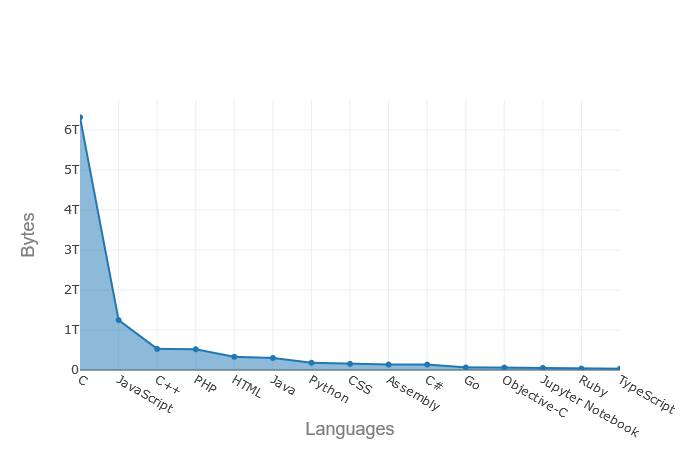
\includegraphics{newplot1.png}
\caption{*QUICK NOTE: B stands for Billion not bytes, i.e 36.48B is
36.48 Billion Bytes thus 36GB}
\end{figure}

    Analyzing byte data from GitHub we see C dominate in the amount with 6.3
TerraBytes of code hosted on the GitHub service. Looking over
Repositories that use the C language one of Github's most popular and
contributed repository is almost 100\% written in C, Linux. Linux the
UNIX based OS and it's kernel is hosted on GitHub with so many
contributers it displays an infinite amount of contributers in its
stats. Since Linux is an OS it is bound to have many C files and in turn
bytes as well, but Linux is not the only C repo, in the top 15 langauges
graph, it shows there are almost 300k projects written in C language and
possibly more. Coming in a far second is JavaScript, GitHub's most
popular language at 1.25 Terabytes of code written amongst the 1.11
Million Javascript projects on Github. We also see other popular
langagues like Python, Java, HTML, and PHP in that list. CSS GitHub's
second most popular language only has about 155 Gb of data, but it's a
style sheet language mainly unlike the rest of the languages up there.

    \subsection{15 Languages that use the Least Amount of
Bytes}\label{languages-that-use-the-least-amount-of-bytes}

    We did the same here except looked at the least amount of bytes:

\begin{Shaded}
\begin{Highlighting}[]
\KeywordTok{SELECT}
\NormalTok{  name,}
  \FunctionTok{SUM}\NormalTok{(bytes) }\KeywordTok{AS}\NormalTok{ totalBytes}
\KeywordTok{FROM}
\NormalTok{  `bigquery-public-data.github_repos.languages` }\KeywordTok{AS}\NormalTok{ l,}
\NormalTok{  UNNEST(l.LANGUAGE)}
\KeywordTok{GROUP} \KeywordTok{BY}
\NormalTok{  name}
\KeywordTok{ORDER} \KeywordTok{BY}
\NormalTok{  totalBytes}
\KeywordTok{limit} \DecValTok{15}
\end{Highlighting}
\end{Shaded}

\begin{figure}[H]
\centering
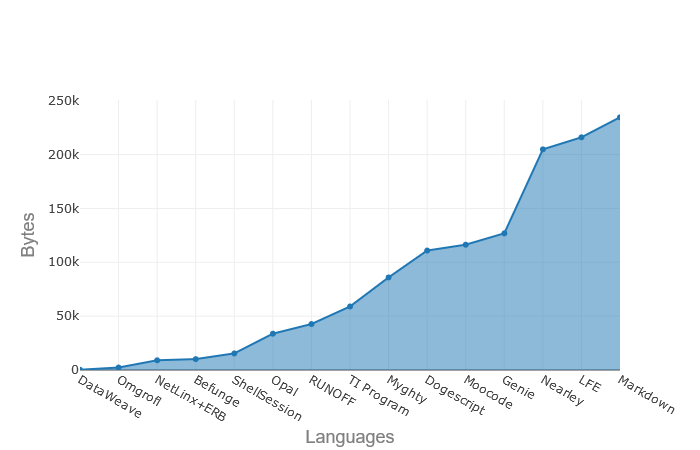
\includegraphics{newplot.png}
\caption{}
\end{figure}

    DataWeave has the least amount of bytes hosted on GitHub. We learned
that Dataweave is a querying language that works with Mule another query
language with Java. One thing that was surprising is a querying language
has least amount of bytes coded compared to DogeScript, a language
developed based in JavaScript, and constantly used and updated.


    \section{Describe possible applications of this data, Including your
ideas for the next
phase}\label{describe-possible-applications-of-this-data-including-your-ideas-for-the-next-phase}

An application for this data is seeing what type of programs use more
storage than others allowing a system administrator to give certain
users more storage based on their favorite language. One interesting
application will be seeing which libraries are commonly used (also see
what type of libraries are most commonly used like reading json/csv
files, machine learning, etc.) and can go a step further and seeing what
are the top 10 libraries for each language for each year. We will be
using this data to predict which languages will be expected to be used
the most in 2018 and 2019. Since we also get information like commits,
we can use this data to see average commits, average time between
commits, and see average lifetime of a repository. We are also able to
see contents of every file in any public repository, so we can use the
contents to teach a machine learning algorithm to tell the difference
between python and javascript or between java and c++, etc.

    \section{Machine Learning - Language
Interpreting}\label{machine-learning---language-interpreting}

    We are also able to see contents of every file in any public repository,
so we can use the contents to teach a machine learning algorithm to tell
the difference between python and javascript or between java and c++,
etc. For this process we went through we gathered the data from the
Github's dataset on Google where we looked at both their \texttt{files}
table and \texttt{content} table. We had to \texttt{JOIN} both tables
based on file ids so we could get filenames and content together. From
there we decided for our machine learning algorithm we would use
Decision Trees to train our machine in recognizing the 8 most popular
langauges which were Java, C, C++, C\#, Objective-c, Python, Ruby, and
Javascript. A problem with gathering the contents was all contents we
got were a mb or less which is a problem as many languages split their
code on many files so many of their files are smaller than normal.

We used regex to create features since programming languages require a
structure to tell one apart from another and all features we used were
boolean (does this language feature the exact structure or not). For
example, Java, C, C++, and many other oop languages share the same for
loop structure but have other distinct features that can differentiate
each one like their print statements. One problem which is hard to avoid
is small programs that share the same structure as other languages but
without the distinct features which can cause an incorrect label. One
way to fix this is to require a certain number of lines to increase the
chance of a distinct feature occurring but even then it could still
fail. One could expand the number of languages simply by adding more
features but eventually the number of features would be cumbersome and
we would have to start combining similar features together. A practical
application for this would be creating a compiler that can detect
certain program structures and allow a user to mix different languages
together like declare an Java array then use a python for loop on it.
Another more complex application would be using these features to try to
reengineer the compiler (or interpreter) and create another machine
learning model (most likely a neural network) to allow even a user who
knows nothing about compilers to create a language based off examples of
it's code. 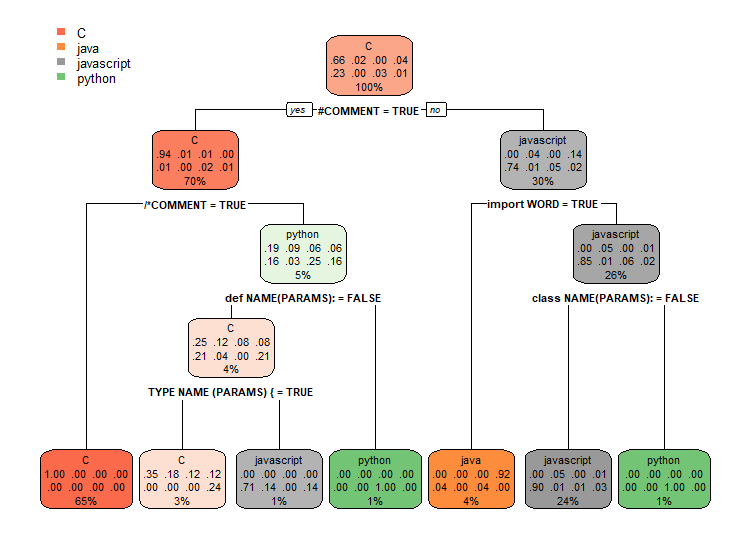
\includegraphics{Rplot.png}

    \section{Conclusion}\label{conclusion}

After spending a semester with this data we've gained some interesting
insights. In terms of programming languages, there are a lot. People
code in obscure languages like DogeScript, Glyph, Opal all of these
languages we've never even heard of before. The big languages are still
the most popular in terms of usage but it's surprising for one to see C
dominate in terms of size in GitHub's platform. In terms of machine
learning, many languages share same features yet have small distinct
features that make them them different. For example many languages share
similar \texttt{For} loop structures, but have different \texttt{print}
statement structures.

Whilst working on this project we faced many challenges. In terms of
gathering data Github's API service provided many limitations in what we
could get, and the rate we could get the data at(API call limit was at
5000 per hour). This made manually running our fetching programs
difficult as we couldn't set up a schedule to run our programs. But with
the responses in JSON format, converting our data to a analyzable CSV
was quite easy with the JSON's great structure and CSV converter
libraries that NodeJS has in npm. BigQuery our biggest source of data
had a monetary impedment where we would need to pay \$5 per every
terabyte queried from their service. GitHub's dataset was over 3
Terabytes total, tables sizes varied. In terms of machine learning we
realized using a bag of words approach using a neural network made it
impossible to get decent accuracy due to unique syntax structure of each
of these langauges we were predicting. Instead we found creating
features using RegEX(Regular Expressions) and associating them on a
decision tree. In terms of bias we encountered more C files in our
dataset than other languages giving it a better overall accuracy than
other languages.

The data set was so large so there is a lot we wish we could do if we
had more time. For one we would try to figure out why one language is
more popular than others in given scenarios. Also GitHub hosts a lot
more information on user activity and collaboration which is something
we would have liked to explore in more depth, i.e which language is
collaborated on more than others and understand why.

Overall, we had a lot of fun analyzing and creating a machine learning
algorithm, especially one that could predict languages. We hope to take
what we learned and maybe even continue this research and analysis
outside of this Introduction Course.

    \subsection{Acknowledgments}\label{acknowledgments}

\begin{itemize}
\tightlist
\item
  \href{https://github.com/octokit/rest.js}{Github API (js)}
\item
  \href{https://www.npmjs.com/package/csv}{csv (js)}
\item
  \href{https://www.npmjs.com/package/jsonfile}{jsonfile (js)}
\item
  \href{https://bigquery.cloud.google.com/dataset/bigquery-public-data:github_repos}{Github
  data (BigQuery)}
\item
  \href{https://plot.ly/python/}{Plotly}
\item
  \href{https://www.rstudio.com/}{Rstudio}
\item
  \href{https://cran.r-project.org/web/packages/rpart/index.html}{Rpart}
\item
  \href{https://cran.r-project.org/web/packages/rpart.plot/index.html}{Rpart.plot}
\end{itemize}


    % Add a bibliography block to the postdoc
    
    
    
    \end{document}
